%!TEX root = tfg.tex
\chapter{Marco teórico}

\begin{abstract}
Este capítulo presenta los fundamentos tecnológicos sobre los que se apoya el proyecto. Se describen las herramientas y sistemas utilizados (ROS2, Gazebo, Nav2, SLAM, AMCL y la plataforma TurtleBot4) con el objetivo de contextualizar las decisiones de diseño e implementación adoptadas a lo largo del trabajo.
\end{abstract}

\section{ROS2: el sistema operativo del robot}

\begin{figure}[H]
    \centering
    
\includegraphics[width=0.4\textwidth]{figures/logos/ros2_logo}
    \caption{Logo de ROS2.}
    \label{fig:logo_ros2}
\end{figure}

ROS2 (Robot Operating System 2)\cite{macenski2022ros2} es un marco de desarrollo de software de código abierto ampliamente utilizado en robótica. A diferencia de su predecesor ROS1, cuyo soporte finalizó en mayo de 2025 con la distribución Noetic, ROS2 fue diseñado desde cero para entornos de producción, con soporte para comunicaciones en tiempo real, sistemas multi-robot y arquitecturas distribuidas.

Su modelo de comunicación se basa en \textbf{nodos} independientes que intercambian información mediante tres mecanismos principales:

\begin{itemize}
    \item \textbf{Topics:} canal de comunicación asíncrono de tipo publicador/suscriptor. Un nodo publica mensajes en un topic y cualquier nodo suscrito los recibe. Es el mecanismo más habitual para datos continuos como lecturas de sensores o comandos de velocidad.
    \item \textbf{Services:} comunicación síncrona de tipo petición/respuesta. El cliente envía una petición y espera la respuesta del servidor antes de continuar.
    \item \textbf{Actions:} similar a los services pero para tareas de larga duración. Permiten enviar un objetivo, recibir retroalimentación periódica sobre el progreso y obtener el resultado final cuando la tarea termina. En este proyecto se utilizan para enviar goals de navegación a Nav2.
\end{itemize}

Este proyecto utiliza la distribución \textbf{ROS2 Humble Hawksbill}\cite{ros2_humble}, lanzada en mayo de 2022 con soporte de largo plazo (LTS) hasta mayo de 2027. Es la distribución oficial para Ubuntu 22.04 y la que los paquetes del TurtleBot4 soportan de forma nativa. En 2026, el ecosistema ROS2 ha evolucionado con distribuciones más recientes como Jazzy Jalisco (2024) y Kilted Kaiju (2025), pero Humble sigue siendo la referencia estable más utilizada en entornos académicos e industriales.

\section{Gazebo: simulación de robots}

\begin{figure}[H]
    \centering
    \begin{minipage}{0.3\textwidth}
        \centering
        
\includegraphics[width=\textwidth]{figures/logos/gazebo_classic_logo}
        \caption{Logo de Gazebo Classic.}
        \label{fig:logo_gazebo_classic}
    \end{minipage}
    \hfill
    \begin{minipage}{0.3\textwidth}
        \centering
        
\includegraphics[width=\textwidth]{figures/logos/ignition_gazebo_logo}
        \caption{Logo de Ignition Gazebo (New Gazebo).}
        \label{fig:logo_ignition}
    \end{minipage}
\end{figure}

Gazebo\cite{koenig2004gazebo} es el simulador de robótica de referencia en el ecosistema ROS2. Permite modelar robots, sensores y entornos físicos con física realista, lo que facilita el desarrollo y validación de algoritmos sin necesidad del hardware real.

Es importante distinguir entre las dos versiones del simulador:

\begin{itemize}
    \item \textbf{Gazebo Classic} (gazebo7--gazebo11): la versión original, lanzada en 2002 y descontinuada en enero de 2025.
    \item \textbf{New Gazebo} (anteriormente Ignition Gazebo): una reescritura completa desarrollada por Open Robotics. Las versiones principales son Citadel, Fortress, Garden y Harmonic. En 2022 el proyecto recuperó el nombre ``Gazebo'', abandonando la marca Ignition.
\end{itemize}

En este proyecto se utiliza \textbf{Ignition Gazebo Fortress}\cite{ignition_fortress}, que es la versión compatible con ROS2 Humble y los paquetes oficiales del TurtleBot4. Fortress ofrece soporte para sensores como LiDAR y cámaras de profundidad, física de contacto realista y un sistema de plugins extensible que permite simular el comportamiento del Create3 con fidelidad suficiente para el desarrollo de algoritmos de navegación.

\section{TurtleBot4 y Create3}

\begin{figure}[H]
    \centering
    \begin{minipage}{0.3\textwidth}
        \centering
        
\includegraphics[width=\textwidth]{figures/logos/turtlebot4_logo}
        \caption{Logo del TurtleBot4.}
        \label{fig:logo_turtlebot4}
    \end{minipage}
    \hfill
    \begin{minipage}{0.3\textwidth}
        \centering
        
\includegraphics[width=\textwidth]{figures/logos/create3_logo}
        \caption{Logo del iRobot Create3.}
        \label{fig:logo_create3}
    \end{minipage}
\end{figure}
\begin{figure}[H]
    \centering
    \begin{minipage}{0.7\textwidth}
        \centering
        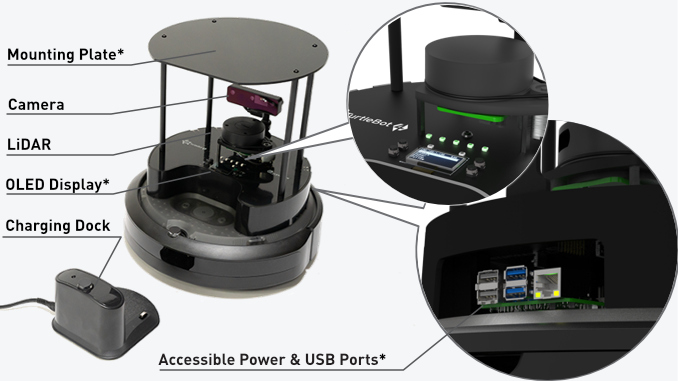
\includegraphics[width=\textwidth]{figures/diagrams/turtlebot4_standard_diagram}
        \caption{Diagrama del TurtleBot4 Standard.}
        \label{fig:diagram_turtlebot4}
    \end{minipage}
\end{figure}

El \textbf{TurtleBot4}\cite{turtlebot4_docs} es una plataforma robótica móvil desarrollada por Clearpath Robotics en colaboración con iRobot, diseñada específicamente para investigación y para aprendizaje con ROS2. Combina una base móvil diferencial, sensores de proximidad, un LiDAR 2D y una cámara de profundidad OAK-D, todo integrado con soporte nativo para ROS2 Humble.

La base del robot es el \textbf{iRobot Create3}\cite{create3_docs}, que hereda el chasis del conocido robot aspirador Roomba. El Create3 incorpora su propio firmware con comportamientos de seguridad integrados, como la detección de bordes, el límite de velocidad máxima de 0,306\,m/s y el \textit{safety timeout} que detiene el robot si deja de recibir comandos de velocidad; que son igualmente reproducidos en la simulación de Ignition Gazebo, lo que garantiza coherencia entre el comportamiento simulado y el del robot real.

En este proyecto se utiliza el modelo \textbf{TurtleBot4 Standard}, que incluye la cámara de profundidad OAK-D Lite además del LiDAR. El sensor principal para la navegación es el \textbf{RPLIDAR A1}, un LiDAR 2D con rango de 12 metros y 360 grados de cobertura que proporciona las lecturas de distancia necesarias para SLAM y la construcción del costmap de Nav2.

\section{SLAM y localización}

\textbf{SLAM} (Simultaneous Localization And Mapping)\cite{durrant2006slam} es la técnica que permite a un robot construir un mapa de su entorno al mismo tiempo que se localiza en él, sin necesidad de un mapa previo. En el contexto de este proyecto, el SLAM se utilizaría para generar el mapa del entorno en una fase inicial, sobre el cual Nav2 planificaría posteriormente las trayectorias.

El paquete utilizado en el ecosistema ROS2 Humble es \textbf{slam\_toolbox}\cite{slam_toolbox}, que implementa un SLAM basado en grafos con corrección de cierres de bucle (\textit{loop closure}). Sin embargo, durante el desarrollo se encontraron limitaciones significativas al intentar ejecutar SLAM en simulación: la discrepancia entre el \texttt{frame\_id} del scan publicado por el LiDAR (\texttt{turtlebot4/rplidar\_link/rplidar}) y el árbol de transformadas TF del simulador, combinada con la velocidad de simulación reducida ($\approx$20\% de la velocidad real en el hardware de desarrollo), impidió que \texttt{slam\_toolbox} procesara los scans correctamente. Como solución, se adoptó el \textbf{mapa pregenerado} del entorno de almacén incluido en los paquetes oficiales del TurtleBot4.

\textbf{AMCL} (Adaptive Monte Carlo Localization)\cite{fox1999amcl} es el algoritmo de localización utilizado por Nav2 cuando ya se dispone de un mapa. Implementa un filtro de partículas en el que cada partícula representa una hipótesis de posición y orientación del robot en el mapa. En cada iteración, el algoritmo compara las lecturas del LiDAR con lo que el robot debería ver desde cada hipótesis, reforzando las partículas más consistentes con los datos reales y eliminando las menos probables. Con el tiempo, las partículas convergen hacia la posición real del robot.

Las figuras~\ref{fig:amcl_1}, \ref{fig:amcl_2} y \ref{fig:amcl_3} muestran la evolución del enjambre de partículas de AMCL durante los primeros segundos de navegación en el entorno de simulación: al arrancar, las partículas están dispersas en una zona amplia del mapa; conforme el robot se mueve y el LiDAR recibe nuevas lecturas, las partículas convergen progresivamente hacia la posición real.

\begin{figure}[H]
    \centering
    \begin{minipage}{0.32\textwidth}
        \centering
        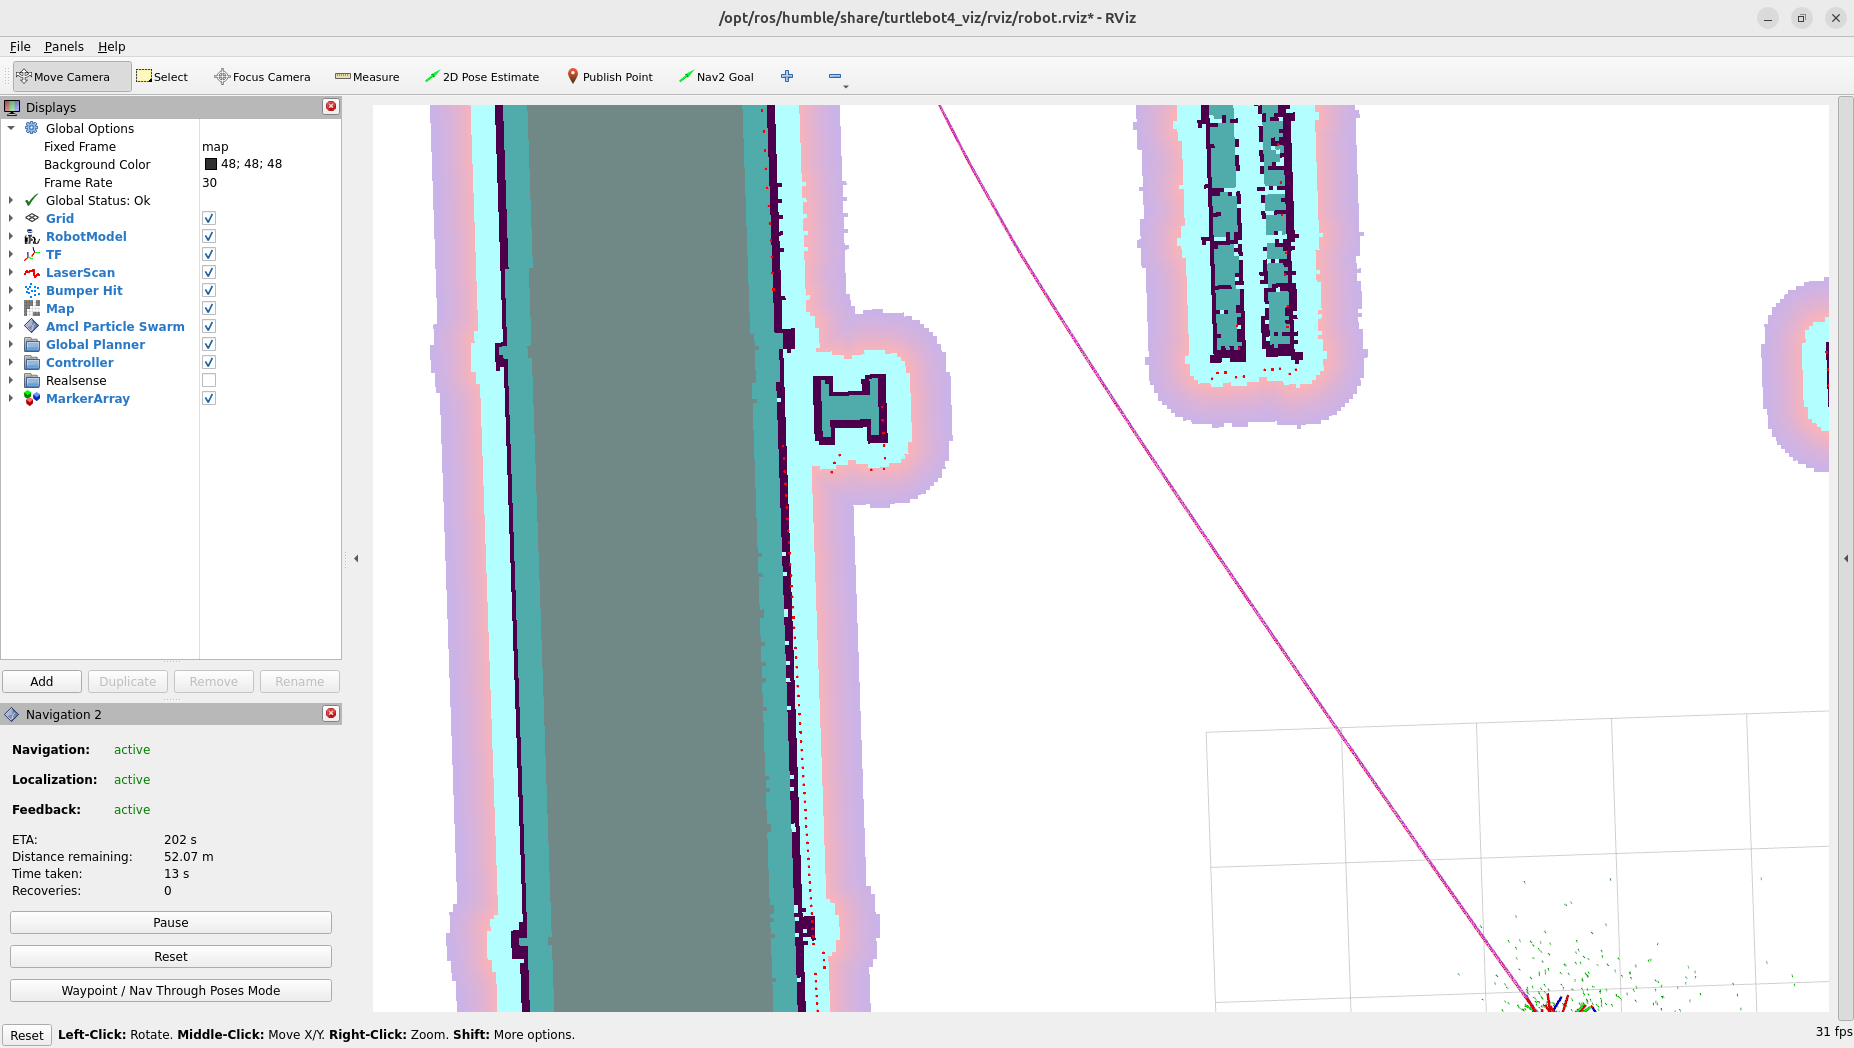
\includegraphics[width=\textwidth]{figures/screenshots/puntos-lidar_1}
        \caption{Partículas AMCL dispersas al inicio (t=13\,s).}
        \label{fig:amcl_1}
    \end{minipage}
    \hfill
    \begin{minipage}{0.32\textwidth}
        \centering
        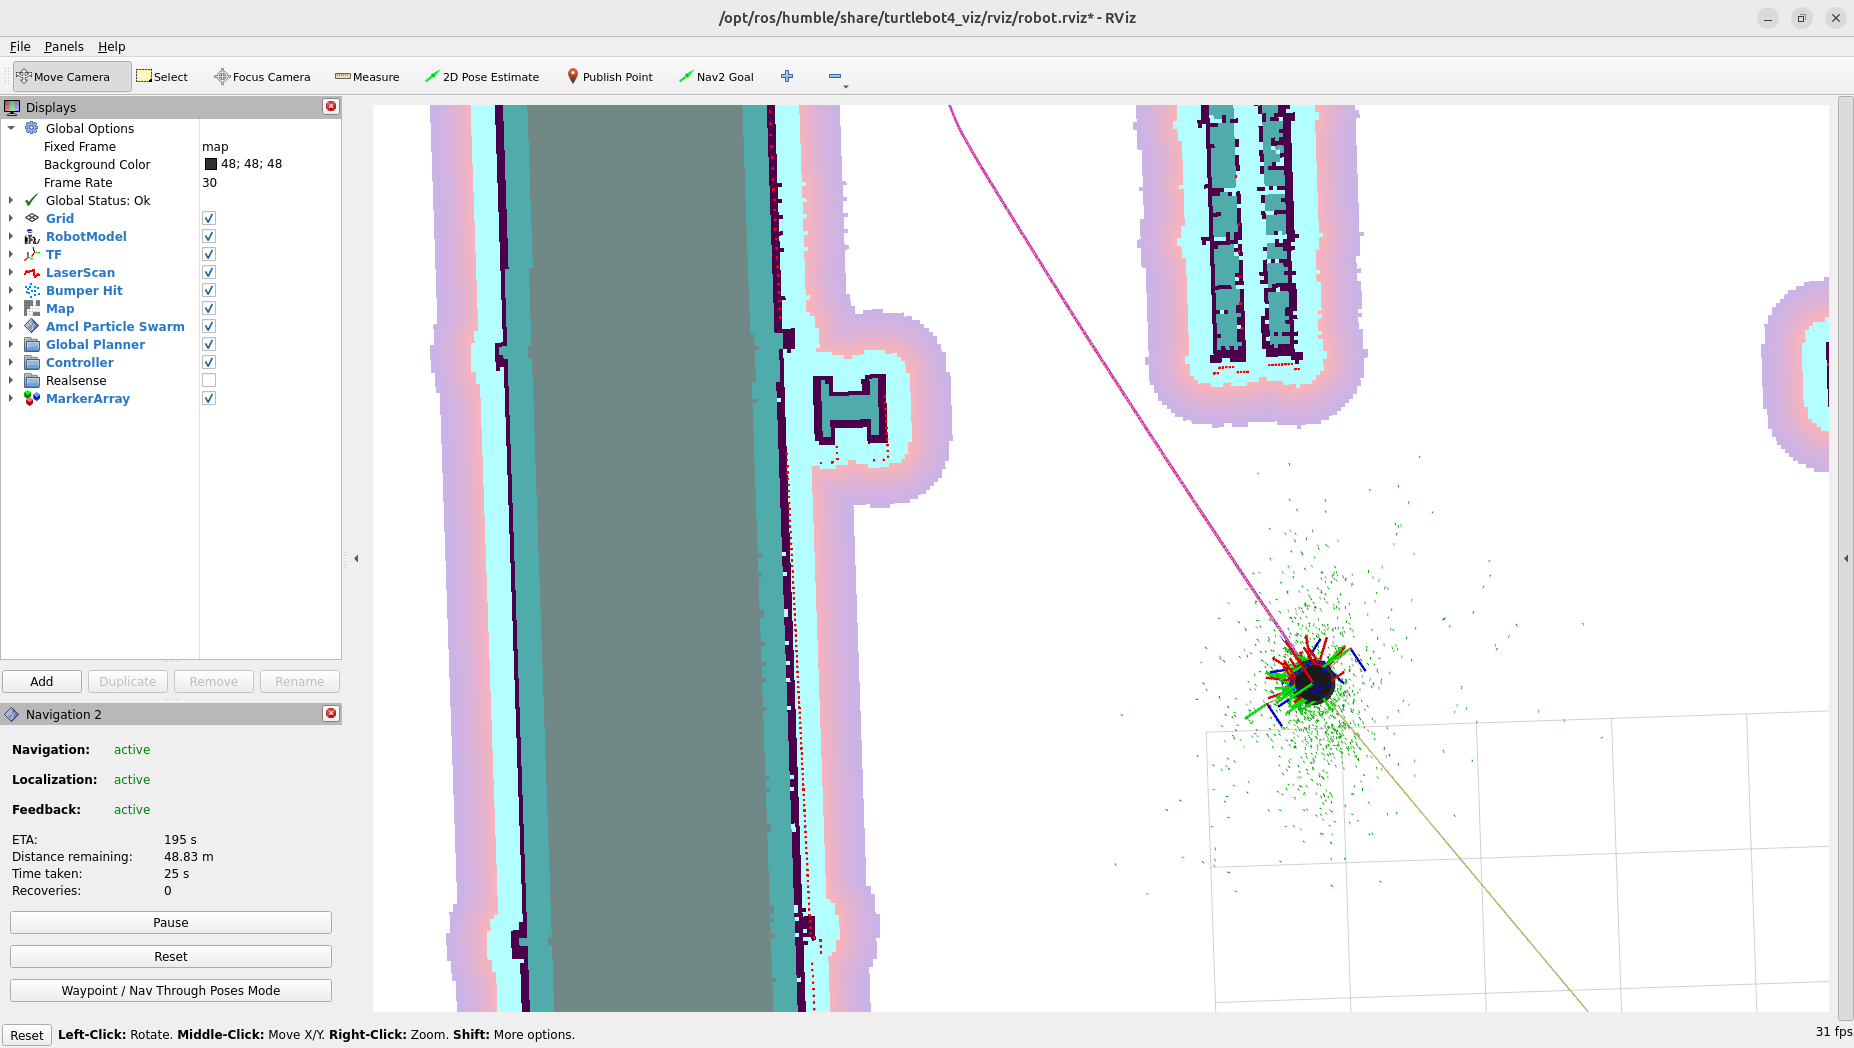
\includegraphics[width=\textwidth]{figures/screenshots/puntos-lidar_2}
        \caption{Partículas convergiendo (t=25\,s).}
        \label{fig:amcl_2}
    \end{minipage}
    \hfill
    \begin{minipage}{0.32\textwidth}
        \centering
        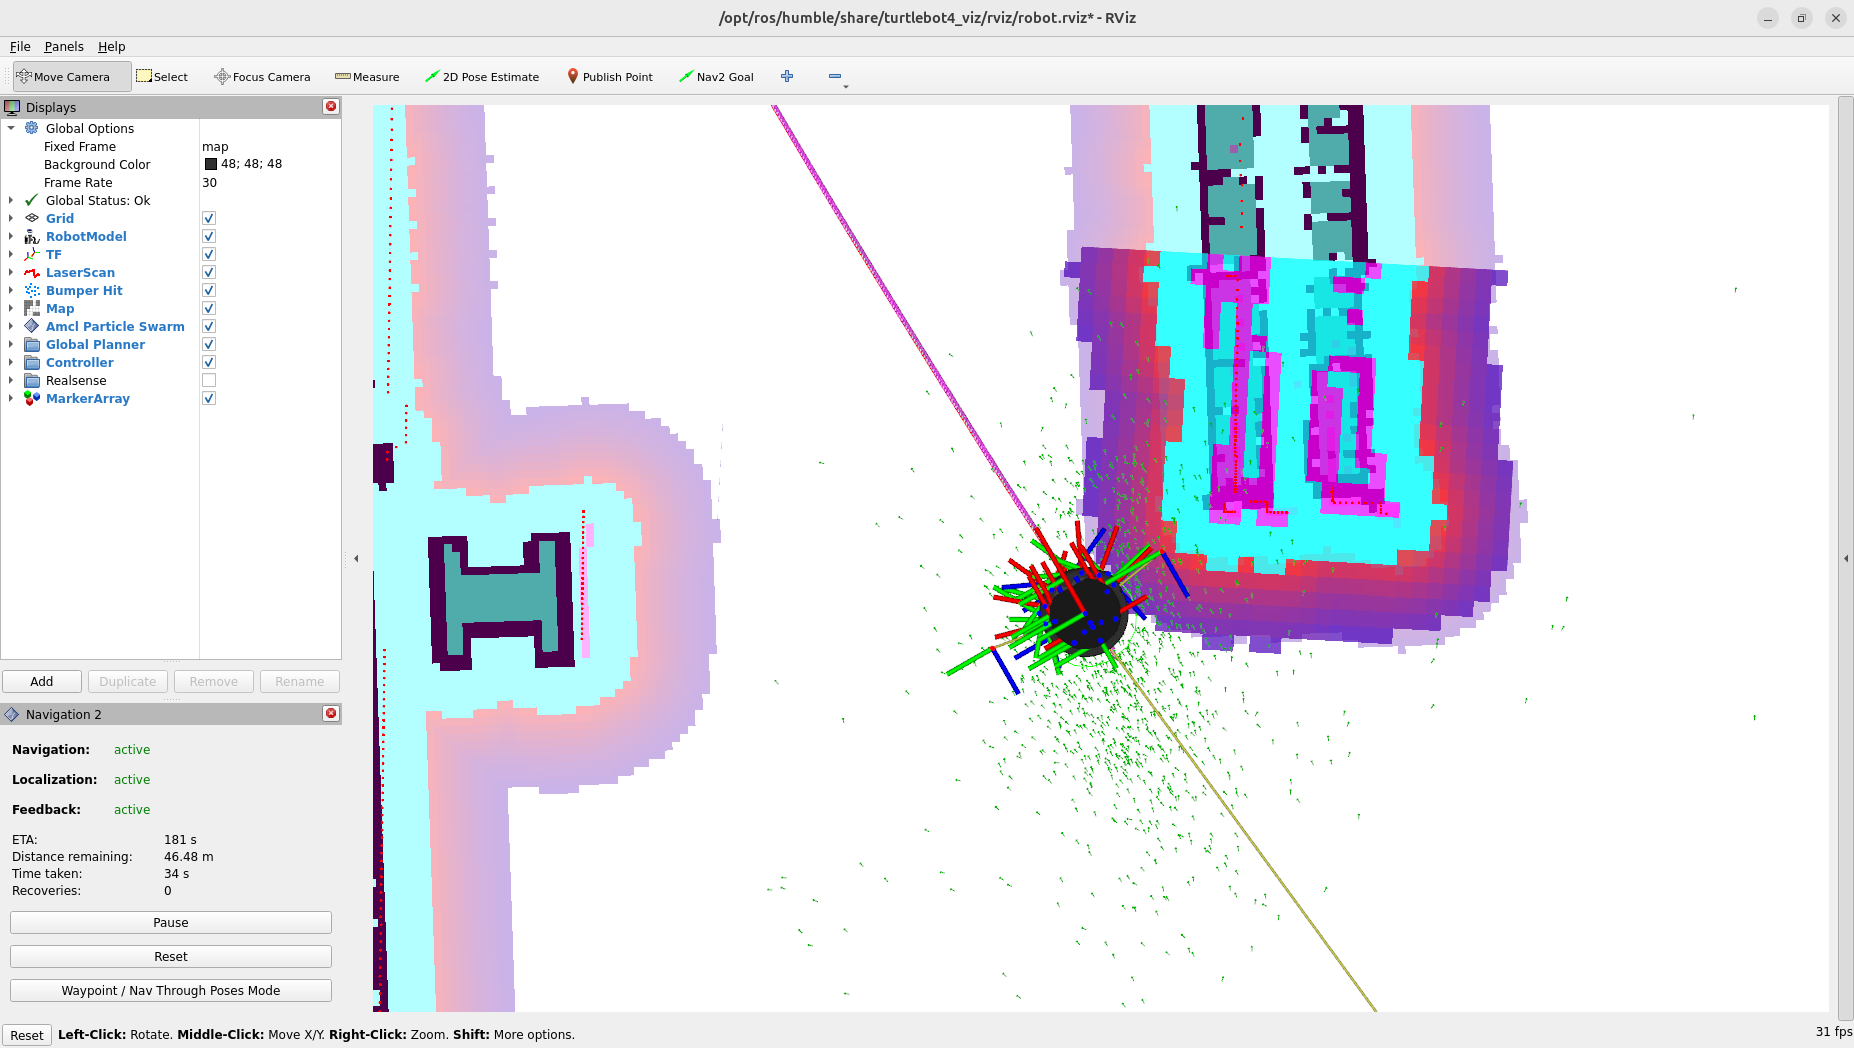
\includegraphics[width=\textwidth]{figures/screenshots/puntos-lidar_3}
        \caption{Partículas concentradas en la pose real (t=34\,s).}
        \label{fig:amcl_3}
    \end{minipage}
\end{figure}

Para inicializar correctamente AMCL es necesario proporcionar una estimación de la pose inicial del robot en el mapa. En este proyecto, este paso se ha automatizado mediante un \texttt{TimerAction} en el launch file que publica la pose inicial en el topic \texttt{/initialpose} al arrancar el sistema.

\section{Nav2: el stack de navegación}

\begin{figure}[H]
    \centering
    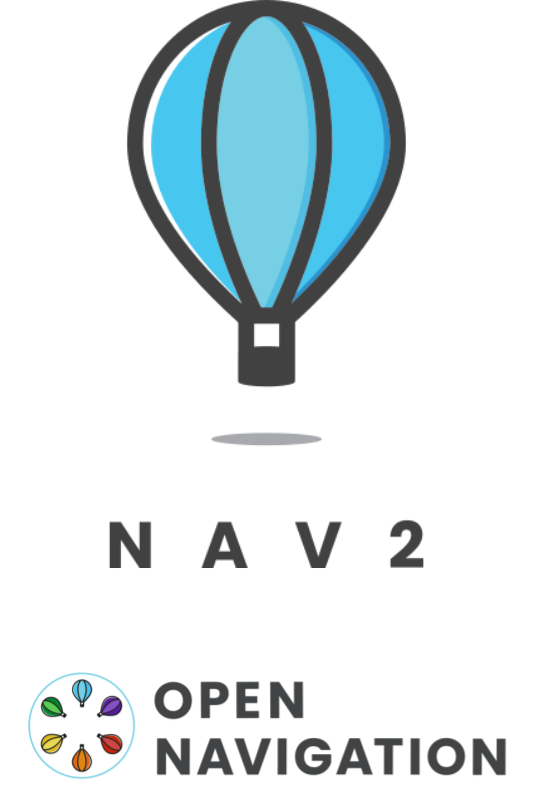
\includegraphics[width=0.2\textwidth]{figures/logos/nav2_logo}
    \caption{Logo de Nav2.}
    \label{fig:logo_nav2}
\end{figure}

\textbf{Nav2} (Navigation2)\cite{macenski2020nav2}\cite{nav2_docs} es el stack de navegación autónoma de referencia en ROS2. Sucesor del \texttt{move\_base} de ROS1, Nav2 proporciona una arquitectura modular y extensible que gestiona todo el proceso de navegación: desde la localización hasta la ejecución de trayectorias, pasando por la planificación global y local y los comportamientos de recuperación ante situaciones de bloqueo.

Sus componentes principales son el \textbf{planificador global} (\texttt{planner\_server}), que calcula la ruta completa desde el origen hasta el destino utilizando el mapa estático; el \textbf{planificador local} o controlador (\texttt{controller\_server}), que genera los comandos de velocidad en tiempo real para seguir la ruta evitando obstáculos dinámicos; y el \textbf{servidor de comportamientos} (\texttt{behavior\_server}), que implementa las estrategias de recuperación como girar sobre sí mismo o retroceder cuando el robot se atasca.

La elección y configuración del planificador global es el elemento central de este trabajo. Nav2 permite cambiar el algoritmo de planificación mediante un sistema de \textit{plugins}, lo que hace posible comparar distintos algoritmos sobre la misma plataforma y en las mismas condiciones. Los algoritmos evaluados y su configuración se describen en detalle más adelante.
